\section{Encapsulation}
Encapsulation is one of the core principles of object-oriented programming. Preserving encapsulation boundaries between objects facilitates reasoning about safety properties like memory safety, data race freedom, safe modification of object implementation.
%Safety is an overloaded term and has been used in the context of both language and program. 
For example, Java is termed as a memory-safe language because it hides memory pointers behind object references which provide safe access to objects. This turns out to be important in order to preserve object semantics which require access to object state using well-defined interfaces. %Another perceived dimension to Java's safety is type-safety. We do not intend to discuss Java's safety features here but we try to convey the point that safety is a broad term. 

%In the context of programs, safety properties describe invariants that should hold in each state of program execution. These are usually properties about semantics of the program rather than a programming model or language.


In the context of the Actor model of programming, we group two core properties of the model under Actor encapsulation. The first one being that there is no shared state among actors. Secondly, an actor can access the state of another actor only by message-passing.

It is very tempting to ignore these semantics in the quest of an efficient implementation of Actor semantics. The temptation is stronger in the case of a library implementation compared to a language implementation. For example, in order to ensure that an actor is unable to access the state of another actor directly, a language may use an abstraction like mailbox address or a channel but use direct references in the compiled code for efficiency. This is similar to how Java uses object references to abstract away pointers. In an actor library, such abstractions (or indirection) have to be resolved at run-time which is more expensive. 

For example, the following code demonstrates violation of one of the core Actor property due to lack of enforcement of Actor encapsulation in the Scala actors library. The main actor, in addition to sending an \code{enter()} message, executes \code{enter()} in its own stack. On a multi-threaded, shared memory implementation of the Actor model, this violates the actor semantics that an actor can only update its local state by processing one message at a time. This can lead to an inconsistent state and manifest into an error.

\makebox[\textwidth]{\hrulefill}
\begin{footnotesize}
\begin{verbatim}
import scala.actors.Actor
import scala.actors.Actor._

object sempahore {
    class SemaphoreActor() extends Actor {
        var MAX = 1;
        var num = 0;

        def act() { 
         loop { react {
                case ("enter") => {
               enter()
                }
                case ("other") => {
                    System.exit(0);
                }
        }}}

        def enter() {
          if (num  < MAX) {
            // critical section
            num = num + 1;
          }
        }
    }

    def main(args : Array[String]) : Unit = {
       var gate = new GateActor()
       gate.start
       gate ! "enter"
       gate.enter
    }
}
\end{verbatim}
\end{footnotesize}
\makebox[\textwidth]{\hrulefill}


We believe that the two aspects of Actor encapsulation are important for writing large-scale Actor programs. It is difficult to provide semantics for and reason about Actor languages not guaranteeing these encapsulation boundaries. \todo {Private conversation with Mirko regarding providing semantics for Scala, which does not guarantee these two aspects.}

In this paper, we focus on how to enforce the property \emph{in a library implementation} that an actor cannot directly access methods (or state) of another actor but may only send messages to it. The problem in this respect is that libraries written on top of existing object-oriented languages represent actors as objects, and the host language can not prevent an actor object from directly calling visible methods on another actor object. We believe that the correct approach is to employ indirect addressing through Actor name objects. A new creation and initialization procedure may be required that returns reference to an Actor name object instead of that to an Actor object. When an actor sends a message to the Actor name, the run-time resolves the name to a mailbox and delivers the message.

\begin{figure}%[htb]
\centerline
{
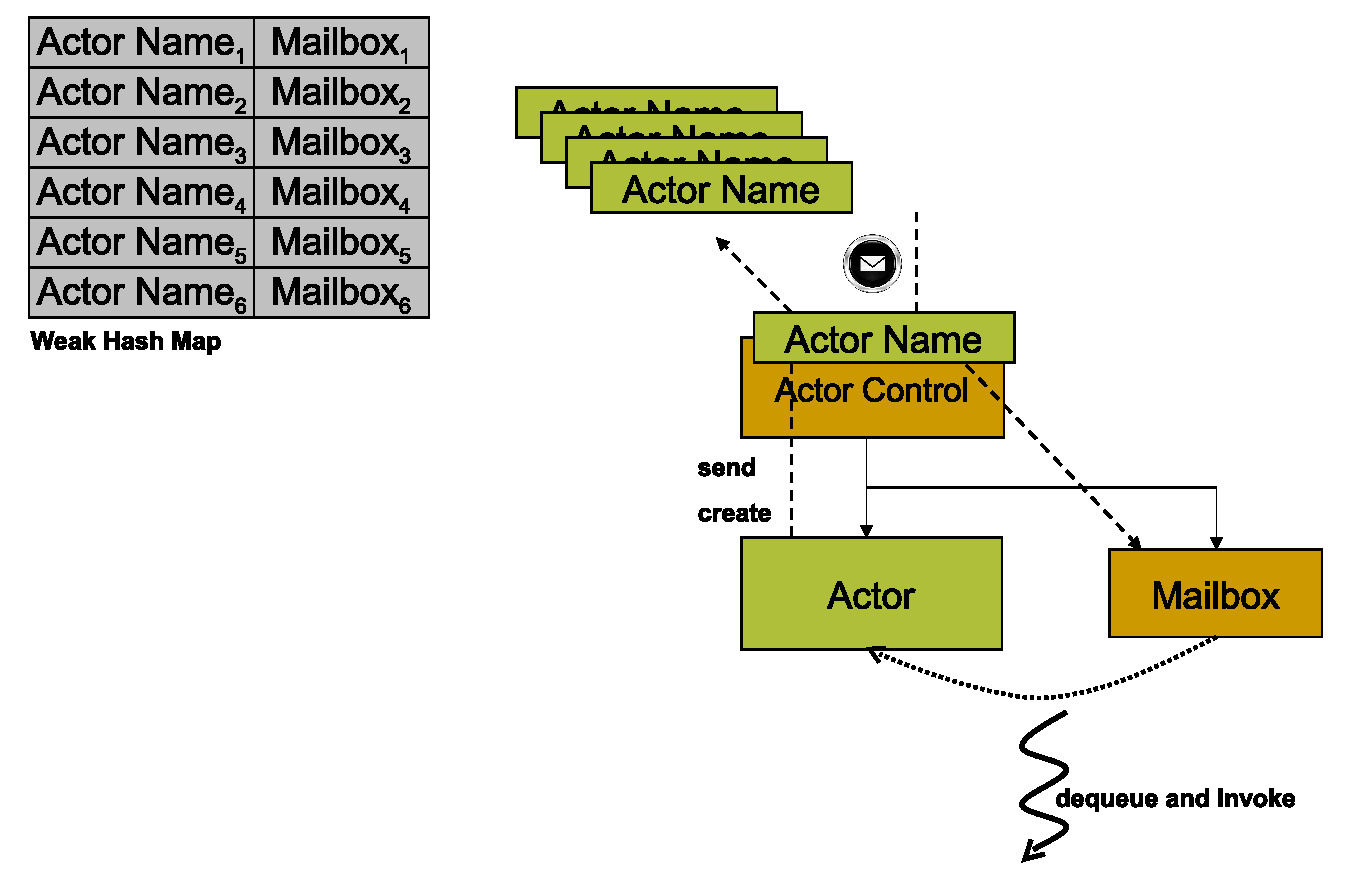
\includegraphics[scale=0.4]{images/escape1.eps}
}
\caption{Actor node using name table with weak references to support encapsulation.}
\label{local_node}
\end{figure}


A simple mechanism is to store the pair of Actor name and mailbox in a hash table. A problem with this approach is that the table can grow unbounded in the absence of an Actor garbage collection mechanism. For example, in Java's implementation of hash tables, each entry in the table would occupy 16 bytes, More importantly though, in the absence of an Actor garbage collection mechanism, an entry in the table means that the actor's state, mailbox and continuation will remain in the memory forever, even if no actor knows its name anymore.


Assuming no support for distributed execution, a more effective solution on platforms with object garbage collection facility, is to use tables with weak references \cite{weakrefs}. Maps with weak references facilitate the following desirable characteristic: the object GC is allowed to remove the Actor name and the corresponding mailbox from the table if the Actor name is not reachable except through the weak reference from inside the table. Hence, the object GC effectively doubles as an Actor GC on a single shared-memory node. An Actor system constituting name tables with weak references is shown in Fig \ref{local_node}

%There is one caveat specific to library implementations; interoperability with existing code can violate encapsulation. For example, a JVM framework which is used by a group of actors and internally employs a stateful singleton object, in effect introduces shared state among actors.

\section{Distributed Execution}
Actor model is based on asynchronous message-passing between independent actors. Hence it provides a uniform model of computation for parallel as well as distributed computing. Apart from programming naturally distributed applications like P2P, sensor networks and Internet computing, distribution is important for parallel performance on scalable multicore architectures. Support for distributed execution is also imperative for mobility.

Distributed execution requires strong references inside the name tables. The reason being that Actors may not be known by any actor inside their node but actors at other hosts may have references to it. Hence, a garbage collector running on the local host may incorrectly remove an entry of an actor from the name table with weak references, and render future messages to the actor from remote actors undeliverable. An Actor system with name tables is shown in Fig \ref{dist_node}.


\begin{figure}%[htb]
\centerline
{
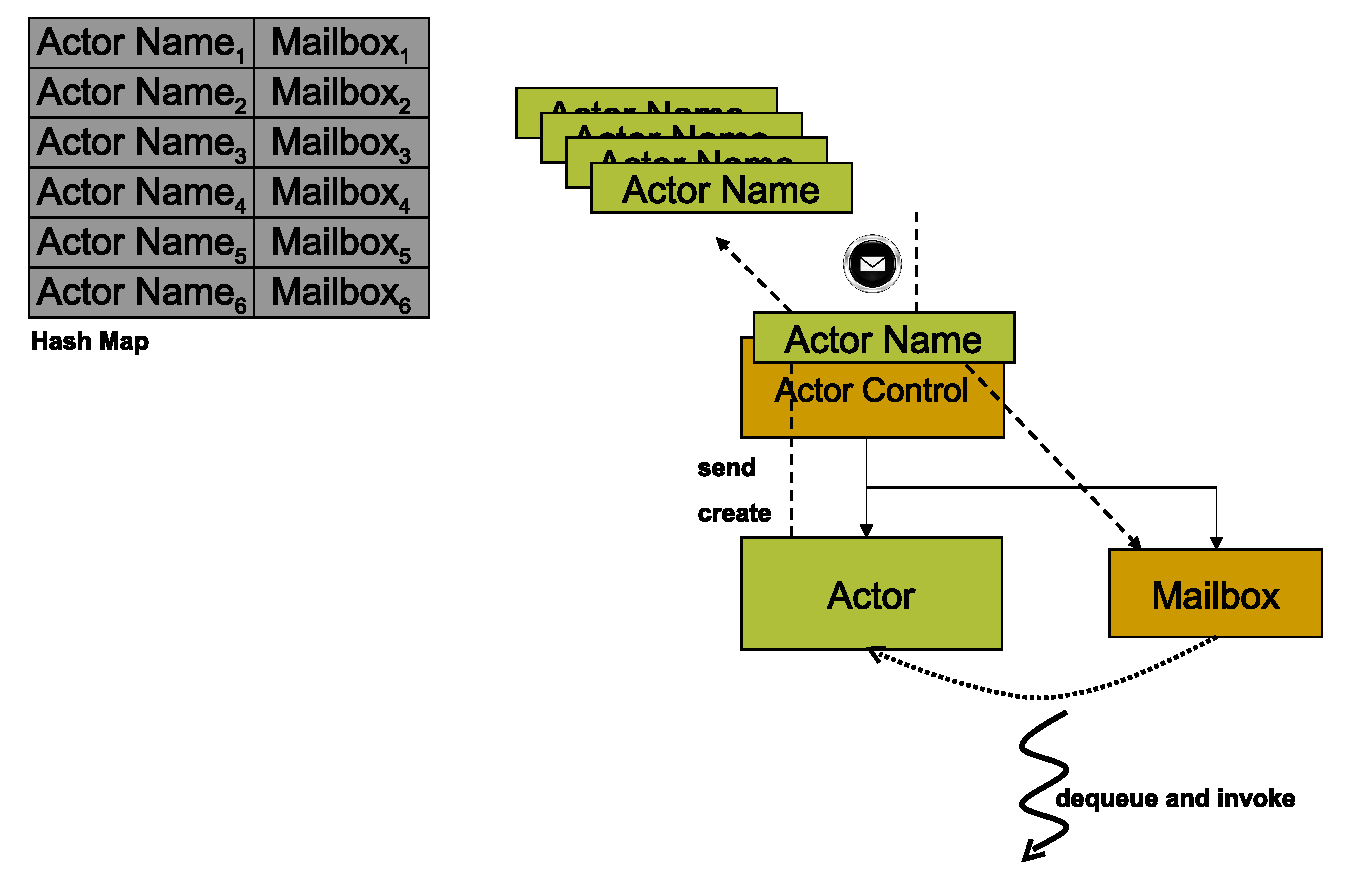
\includegraphics[scale=0.4]{images/escape2.eps}
}
\caption{Actor node with name table to support distributed execution.}
\label{dist_node}
\end{figure}


%\code example - Weather widget talking to weather server

%\subsection{Location Transparency}

\section{Strong Mobility}

Proponents of Actor model emphasize transparent distribution of Actor programs, making the programs elegant and the task of the programmer less arduous. Actor systems should be able to provide facilities like load-balancing and fault-tolerance while keeping a uniform location-independent naming model for programmers. This in turn separates the concern of ``what'' from ``where'' and enables optimizations by the system based on run-time conditions.

Mobility is defined as the ability of computation to move across different nodes. In their seminal work, Fuggetta et al. classify mobility as either strong or weak \cite{mobility}. Strong mobility is defined as the ability of a system to support movement of both code and execution state. Weak mobility, on the other hand, allows movement of only code. Initial state may be transferrable though in weak mobility.

At the system level weak mobility is essential for achieving load-balancing, facilitating fault-tolerance, reconfiguration. Previous work has shown that location transparency and mobility can be essential for achieving scalable performance, specially for dynamic, irregular applications over sparse data structures \cite{jpdc94}. In such applications different stages may require a different distribution of computation. In other cases, the optimal distribution is dependent on run-time conditions such as data and work load. The ability to dynamically redistribute computation requires support for mobility.

We also believe that strong mobility enables declarative exploitation of heterogeneous system resources such as GPUs, DSPs, other task-specific accelerators, high clock frequency cores, (when augmented with discovery services). It leads to elegant programming and simpler control flow.

\makebox[\textwidth]{\hrulefill}
\begin{footnotesize}
\begin{verbatim}

actor MatrixMultiply {
  message start(int N) {
   // Random generation of A, B
   
   migrate("gpu");

   int [][] C = new int [N][N];
   create <N * N> MultiplyActor()<-start(A, B, C);

   migrate("cpu");
   // print C

  }
}

actor MultiplyActor {
  int id;
  message multiply (int [][] A, int [][] B, int [][] C) {
    int i = id % N, j = id / N;
    C[i][j] = A[i][j] * B[i][j];
  }
}

\end{verbatim}
\end{footnotesize}
\makebox[\textwidth]{\hrulefill}


It can also express streaming-code algorithms where the programmer wishes to move code rather than data. In combination with data discovery services, mobile actors can process data in-place. This may be preferable due to privacy reasons or that it is more efficient to move code rather than data. This is quite similar to pipeline processing except that the conceptual model is reversed: transformation actors processing the statically residing data one after the other. Moreover, this model by definition has ownership transfer semantics for messages, which as discussed earlier can be implemented more efficiently.
%Having strong mobility as a primitive helps the programmer e

Mobility is quite natural to the Actor model due to modularity of control and encapsulation. Object-oriented languages may allow mobility at the level of objects but all thread stacks executing methods on the object need to be made aware of this migration. Moreover, when the stack frame require access to the object on a remote node, the execution stack is moved to the remote node, complete the execution of the frame and then migrated back to the original node \cite{walsh2000spm}.


A protocol for supporting mobility in Actor systems has been described in \cite{sc95}. It requires Actor names to be mapped to be mapped to their possible host. Hence, in addition to name table for looking up the Actor state, an Actor system requires another name service that can lookup the host (physical address) of an Actor. An Actor system with name tables is shown in Fig \ref{mobile_node}.

\begin{figure}%[htb]
\centerline
{
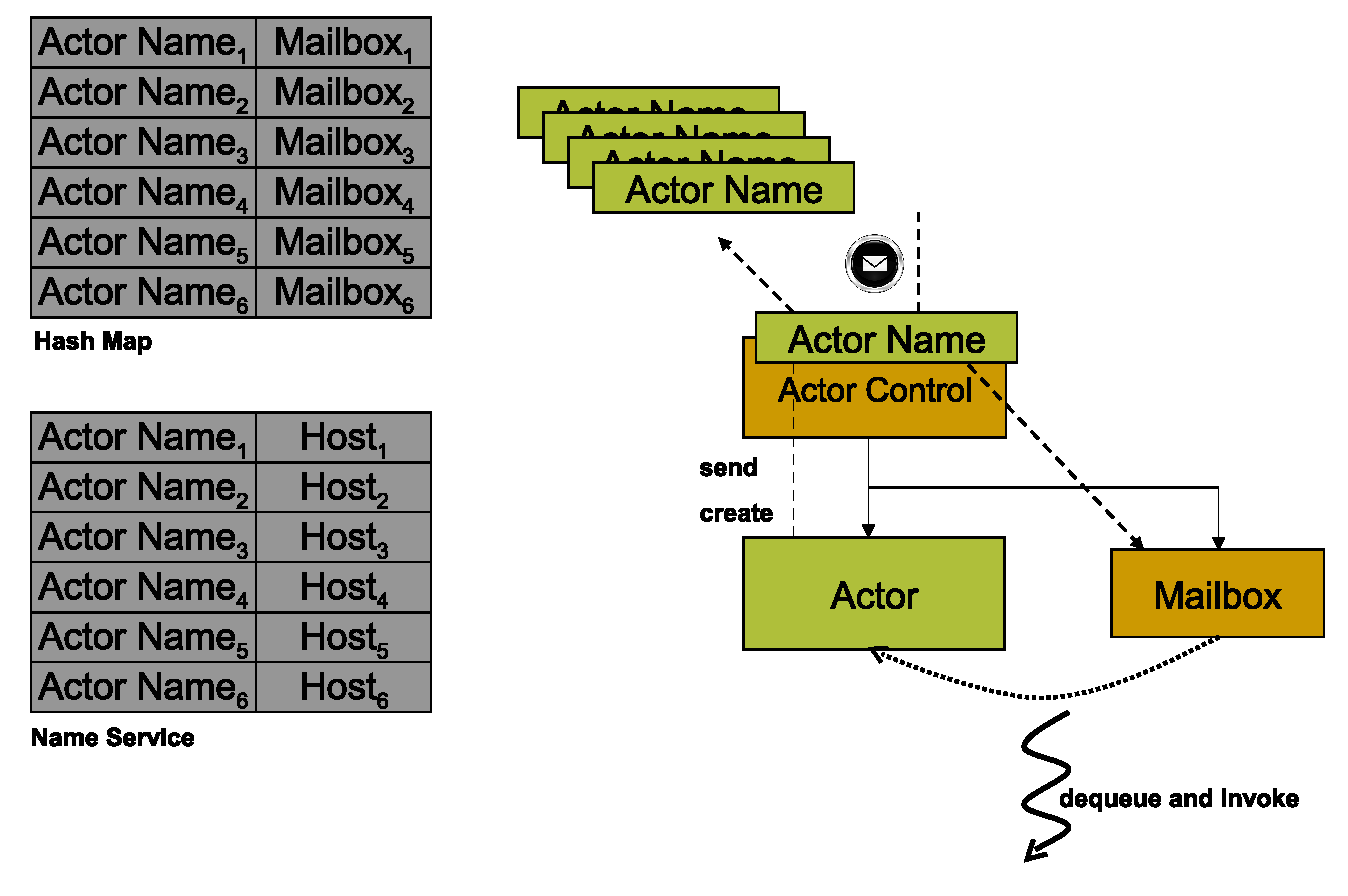
\includegraphics[scale=0.4]{images/escape3.eps}
}
\caption{Actor node with name table and a name service to support mobility}
\label{mobile_node}
\end{figure}
